\section{Background}

\begin{frame}{Background}% {Optional Subtitle}
\begin{block}{Recommendation Fairness}
Consider a service recommendation scenario with capacity constraints, 
some customers may not able to get satisfactory service quality.
%%%
\end{block}

% zlt add description here
\begin{figure}[H]
  \centering
  \subfigure[Shared Bike Recommendation (A previous project at EI333)]{
    \begin{minipage}[t]{0.4\linewidth}
    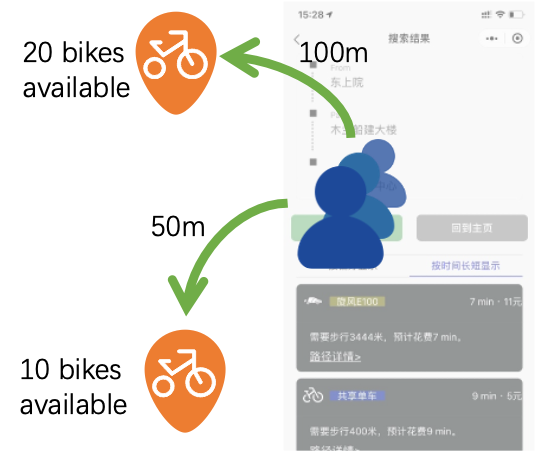
\includegraphics[width=0.9\textwidth]{img/intro_case1.png}
    \end{minipage}
  }
  \hspace{0.2in}
  \subfigure[Restaurant Recommendation]{
    \begin{minipage}[t]{0.4\linewidth}
    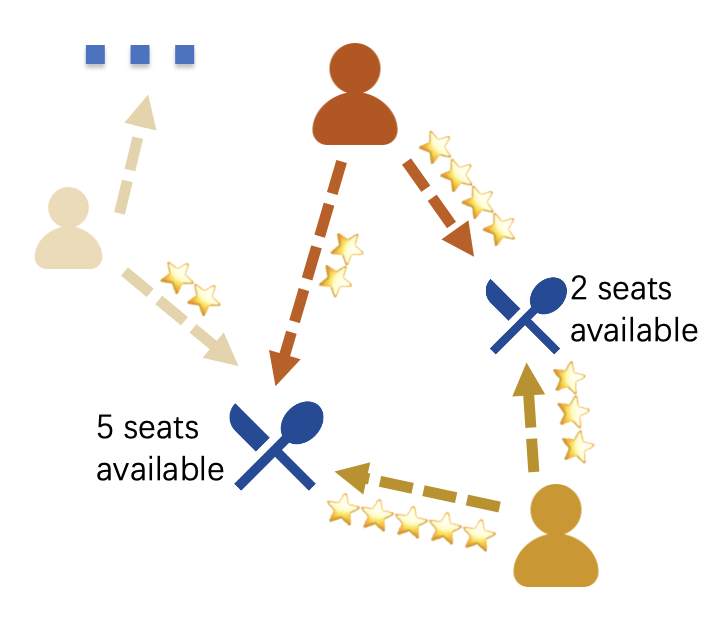
\includegraphics[width=0.9\textwidth]{img/intro_case2.png}
    \end{minipage}
  }
\end{figure}

We need to (1) meet the capacity constraint, (2) ensure individual fairness, (3) maintain recommendation quality.

\end{frame}







\begin{frame}{Background\footnote{Yao Wu, \textbf{Jian Cao}, and Guandong Xu. “FAST: A Fairness Assured Service Recommendation StrategyConsidering Service Capacity Constraint”. In: Service-Oriented Computing, (ICSOC 2020)}}

\begin{block}{FAST: Fairness Assured Service Recommendation Strategy}
\textbf{Significance}
  \begin{enumerate}
      \item Establishing a metric for fairness;
      \item Giving an algorithm to adjust recommendation results to ensure Fairness among users in N rounds while maintaining a high recommendation quality
  \end{enumerate}


 \textbf{Shortcoming}
 \begin{enumerate}
     \item High computational complexity with at least a computation of
$O(n log n)$ per request;
     \item The proposed algorithm can only calculate a global recommendation plan
after all users’ information has been gathered
     
 \end{enumerate}
\end{block}

    
\end{frame}






\begin{frame}{Background}

 \begin{block}{Shortcoming of FAST}
  \begin{enumerate}
     \item High computational complexity with at least a computation of $O(n log n)$ per request;
     \item The proposed algorithm can only calculate a global recommendation plan after all users’ information has been gathered
     \item The analysis of FAST assumes a \textbf{fixed} user set.
     
 \end{enumerate}
 \end{block}


~\\

These Shortcomings hinder FAST from online deployment.
~\\

Our Goal: Establish an Online FAST algorithm.
     \begin{enumerate}
     \item Lower its computing complexity
     \item Give a recommended service whenever it gets a request
     \item Allow users come with a probability
     
 \end{enumerate}
\end{frame}

